\documentclass{beamer}
\usetheme{EastLansing}\usecolortheme{crane}
\usefonttheme{professionalfonts}\useinnertheme{rectangles}
\newcommand{\putfig}[1]{%
	\vspace{0.8em}%
	\centerline{\includegraphics[scale=1]{./figures/#1}}%
	\vspace{0.5em}%
}
\newcommand{\separationline}{%
	\vspace{0.3em}%
	\centerline{----- $*$ ----- $*$ ----- $*$ -----}%
	\vspace{0.3em}%
}
\newcommand{\ratio}{\!:\!}
%<--------------------------------------------------------------------------->%
%%% Column %%%
\usepackage{multicol}  % \begin{multicols*}{3}[例外]字\end{multicols*}
\usepackage[english]{babel}
%<--------------------------------------------------------------------------->%
%%% Enumerate %%%
\usepackage{enumitem}
\setlist{listparindent=\parindent,parsep=0pt,nosep} % paragraph indent 
%<--------------------------------------------------------------------------->%
%%% Math %%%
\usepackage{gensymb,amssymb}
\usepackage{mathrsfs,amsmath} % \mathscr{F}
\usepackage{mathtools} % \stackrel{i.i.d.}{\sim} % \substack{-\\-} % \middle
% \usepackage{centernot}
% \usepackage{accents}
% \usepackage[makeroom]{cancel}
% \newcommand{\two}[2]{\substack{ \text{#1} \\ \text{#2} }}
% \newcommand{\raum}{\phantom{=}{\:\,}}
%<--------------------------------------------------------------------------->%
%%% Page # of # %%%
\usepackage{fancyhdr,lastpage}
\pagestyle{fancy}\renewcommand{\headrulewidth}{0pt}\fancyhf{}
\fancyfoot[C]{\footnotesize 第 \thepage\ 頁 / 共 \pageref{LastPage} 頁}
\fancypagestyle{plain}{\renewcommand{\headrulewidth}{0pt}\fancyhf{}
\fancyfoot[C]{\footnotesize 第 \thepage\ 頁 / 共 \pageref{LastPage} 頁}}
%<--------------------------------------------------------------------------->%
%%% Hyper Reference %%%
\PassOptionsToPackage{hyphens}{url}
\usepackage[hidelinks,colorlinks=true]{hyperref}
% \newcommand{\supref}[1]{\ref{#1} (p.\pageref{#1})}
%<--------------------------------------------------------------------------->%
%%% CJK %%%
\usepackage{xeCJK}
\newcommand{\chmainfont}{GenWanMin TJ L}
\newcommand{\chsansfont}{Noto Sans CJK KR Medium}
\newcommand{\chmonofont}{Noto Sans CJK KR Regular}
\setCJKmainfont{\chmainfont}[BoldFont=\chsansfont,AutoFakeSlant=0.2]
\setCJKsansfont{\chsansfont}[BoldFont=\chsansfont,AutoFakeSlant=0.2]
\setCJKmonofont{\chmonofont}
\xeCJKsetup{PunctStyle=kaiming,CheckFullRight=true}
\setlength{\parindent}{2em}
%<--------------------------------------------------------------------------->%
%%% Punctuation width %%%
\xeCJKsetwidth{、}{0.55em}
\xeCJKsetwidth{,}{0.6em}
\xeCJKsetwidth{:}{0.65em}
\xeCJKsetwidth{;}{0.65em}
\xeCJKsetwidth{。}{0.7em}
\xeCJKsetwidth{・}{0.7em}
\xeCJKsetwidth{〈〉}{0.7em}
\xeCJKsetwidth{《》}{0.7em}
\xeCJKsetwidth{「」}{0.7em}
\xeCJKsetwidth{『』}{0.7em}
\xeCJKsetwidth{【】}{0.7em}
\xeCJKsetwidth{()}{0.7em}
%<--------------------------------------------------------------------------->%
%%% Punctuation Kerning %%%
% Pairs-with-punctuation kerning (after).
\xeCJKsetkern{〉}{、}{0.2em} \xeCJKsetkern{〉}{,}{0.2em} \xeCJKsetkern{〉}{。}{0.2em} \xeCJKsetkern{〉}{;}{0.2em} \xeCJKsetkern{〉}{:}{0.2em} 
\xeCJKsetkern{》}{、}{0.2em} \xeCJKsetkern{》}{,}{0.2em} \xeCJKsetkern{》}{。}{0.2em} \xeCJKsetkern{》}{;}{0.2em} \xeCJKsetkern{》}{:}{0.2em} 
\xeCJKsetkern{」}{、}{0.2em} \xeCJKsetkern{」}{,}{0.2em} \xeCJKsetkern{」}{。}{0.2em} \xeCJKsetkern{」}{;}{0.2em} \xeCJKsetkern{」}{:}{0.2em} 
\xeCJKsetkern{』}{、}{0.2em} \xeCJKsetkern{』}{,}{0.2em} \xeCJKsetkern{』}{。}{0.2em} \xeCJKsetkern{』}{;}{0.2em} \xeCJKsetkern{』}{:}{0.2em} 
\xeCJKsetkern{】}{、}{0.2em} \xeCJKsetkern{】}{,}{0.2em} \xeCJKsetkern{】}{。}{0.2em} \xeCJKsetkern{】}{;}{0.2em} \xeCJKsetkern{】}{:}{0.2em} 
\xeCJKsetkern{)}{、}{0.2em} \xeCJKsetkern{)}{,}{0.2em} \xeCJKsetkern{)}{。}{0.2em} \xeCJKsetkern{)}{;}{0.2em} \xeCJKsetkern{)}{:}{0.2em} 
% Pairs-with-punctuation kerning (before).
\xeCJKsetkern{、}{〈}{0.4em} \xeCJKsetkern{。}{〈}{0.4em} \xeCJKsetkern{,}{〈}{0.4em} \xeCJKsetkern{:}{〈}{0.4em} \xeCJKsetkern{;}{〈}{0.4em}
\xeCJKsetkern{、}{《}{0.4em} \xeCJKsetkern{。}{《}{0.4em} \xeCJKsetkern{,}{《}{0.4em} \xeCJKsetkern{:}{《}{0.4em} \xeCJKsetkern{;}{《}{0.4em}
\xeCJKsetkern{、}{「}{0.4em} \xeCJKsetkern{。}{「}{0.4em} \xeCJKsetkern{,}{「}{0.4em} \xeCJKsetkern{:}{「}{0.4em} \xeCJKsetkern{;}{「}{0.4em}
\xeCJKsetkern{、}{『}{0.4em} \xeCJKsetkern{。}{『}{0.4em} \xeCJKsetkern{,}{『}{0.4em} \xeCJKsetkern{:}{『}{0.4em} \xeCJKsetkern{;}{『}{0.4em}
\xeCJKsetkern{、}{【}{0.4em} \xeCJKsetkern{。}{【}{0.4em} \xeCJKsetkern{,}{【}{0.4em} \xeCJKsetkern{:}{【}{0.4em} \xeCJKsetkern{;}{【}{0.4em}
\xeCJKsetkern{、}{(}{0.4em} \xeCJKsetkern{。}{(}{0.4em} \xeCJKsetkern{,}{(}{0.4em} \xeCJKsetkern{:}{(}{0.4em} \xeCJKsetkern{;}{(}{0.4em}
% Pairwise kerning (back-to-back).
\xeCJKsetkern{〉}{〈}{0.3em} \xeCJKsetkern{〉}{《}{0.3em} \xeCJKsetkern{〉}{「}{0.3em} \xeCJKsetkern{〉}{『}{0.3em} \xeCJKsetkern{〉}{【}{0.3em} \xeCJKsetkern{〉}{(}{0.3em}
\xeCJKsetkern{》}{〈}{0.3em} \xeCJKsetkern{》}{《}{0.3em} \xeCJKsetkern{》}{「}{0.3em} \xeCJKsetkern{》}{『}{0.3em} \xeCJKsetkern{》}{【}{0.3em} \xeCJKsetkern{》}{(}{0.3em}
\xeCJKsetkern{」}{〈}{0.3em} \xeCJKsetkern{」}{《}{0.3em} \xeCJKsetkern{」}{「}{0.3em} \xeCJKsetkern{」}{『}{0.3em} \xeCJKsetkern{」}{【}{0.3em} \xeCJKsetkern{」}{(}{0.3em}
\xeCJKsetkern{』}{〈}{0.3em} \xeCJKsetkern{』}{《}{0.3em} \xeCJKsetkern{』}{「}{0.3em} \xeCJKsetkern{』}{『}{0.3em} \xeCJKsetkern{』}{【}{0.3em} \xeCJKsetkern{』}{(}{0.3em}
\xeCJKsetkern{】}{〈}{0.3em} \xeCJKsetkern{】}{《}{0.3em} \xeCJKsetkern{】}{「}{0.3em} \xeCJKsetkern{】}{『}{0.3em} \xeCJKsetkern{】}{【}{0.3em} \xeCJKsetkern{】}{(}{0.3em}
\xeCJKsetkern{)}{〈}{0.3em} \xeCJKsetkern{)}{《}{0.3em} \xeCJKsetkern{)}{「}{0.3em} \xeCJKsetkern{)}{『}{0.3em} \xeCJKsetkern{)}{【}{0.3em} \xeCJKsetkern{)}{(}{0.3em}
% Pairwise kerning (font-to-back).
\xeCJKsetkern{〈}{〈}{0.2em} \xeCJKsetkern{〈}{《}{0.2em} \xeCJKsetkern{〈}{「}{0.2em} \xeCJKsetkern{〈}{『}{0.2em} \xeCJKsetkern{〈}{【}{0.2em} \xeCJKsetkern{〈}{(}{0.2em}
\xeCJKsetkern{《}{〈}{0.2em} \xeCJKsetkern{《}{《}{0.2em} \xeCJKsetkern{《}{「}{0.2em} \xeCJKsetkern{《}{『}{0.2em} \xeCJKsetkern{《}{【}{0.2em} \xeCJKsetkern{《}{(}{0.2em}
\xeCJKsetkern{「}{〈}{0.2em} \xeCJKsetkern{「}{《}{0.2em} \xeCJKsetkern{「}{「}{0.2em} \xeCJKsetkern{「}{『}{0.2em} \xeCJKsetkern{「}{【}{0.2em} \xeCJKsetkern{「}{(}{0.2em}
\xeCJKsetkern{『}{〈}{0.2em} \xeCJKsetkern{『}{《}{0.2em} \xeCJKsetkern{『}{「}{0.2em} \xeCJKsetkern{『}{『}{0.2em} \xeCJKsetkern{『}{【}{0.2em} \xeCJKsetkern{『}{(}{0.2em}
\xeCJKsetkern{【}{〈}{0.2em} \xeCJKsetkern{【}{《}{0.2em} \xeCJKsetkern{【}{「}{0.2em} \xeCJKsetkern{【}{『}{0.2em} \xeCJKsetkern{【}{【}{0.2em} \xeCJKsetkern{【}{(}{0.2em}
\xeCJKsetkern{(}{〈}{0.2em} \xeCJKsetkern{(}{《}{0.2em} \xeCJKsetkern{(}{「}{0.2em} \xeCJKsetkern{(}{『}{0.2em} \xeCJKsetkern{(}{【}{0.2em} \xeCJKsetkern{(}{(}{0.2em}
% Pairwise kerning (back-to-front).
\xeCJKsetkern{〉}{〉}{0.2em} \xeCJKsetkern{〉}{》}{0.2em} \xeCJKsetkern{〉}{」}{0.2em} \xeCJKsetkern{〉}{』}{0.2em} \xeCJKsetkern{〉}{】}{0.2em} \xeCJKsetkern{〉}{)}{0.2em}
\xeCJKsetkern{》}{〉}{0.2em} \xeCJKsetkern{》}{》}{0.2em} \xeCJKsetkern{》}{」}{0.2em} \xeCJKsetkern{》}{』}{0.2em} \xeCJKsetkern{》}{】}{0.2em} \xeCJKsetkern{》}{)}{0.2em}
\xeCJKsetkern{」}{〉}{0.2em} \xeCJKsetkern{」}{》}{0.2em} \xeCJKsetkern{」}{」}{0.2em} \xeCJKsetkern{」}{』}{0.2em} \xeCJKsetkern{」}{】}{0.2em} \xeCJKsetkern{」}{)}{0.2em}
\xeCJKsetkern{』}{〉}{0.2em} \xeCJKsetkern{』}{》}{0.2em} \xeCJKsetkern{』}{」}{0.2em} \xeCJKsetkern{』}{』}{0.2em} \xeCJKsetkern{』}{】}{0.2em} \xeCJKsetkern{』}{)}{0.2em}
\xeCJKsetkern{】}{〉}{0.2em} \xeCJKsetkern{】}{》}{0.2em} \xeCJKsetkern{】}{」}{0.2em} \xeCJKsetkern{】}{』}{0.2em} \xeCJKsetkern{】}{】}{0.2em} \xeCJKsetkern{】}{)}{0.2em}
\xeCJKsetkern{)}{〉}{0.2em} \xeCJKsetkern{)}{》}{0.2em} \xeCJKsetkern{)}{」}{0.2em} \xeCJKsetkern{)}{』}{0.2em} \xeCJKsetkern{)}{】}{0.2em} \xeCJKsetkern{)}{)}{0.2em}
%<--------------------------------------------------------------------------->%

%<--------------------------------------------------------------------------->%
\title{\textbf{Introduction to \\Generalised Method of Moments}}
\subtitle{Econometrics (2000) Hayashi, Chapter 3}
\author{陳\;捷\hspace{1em}\texttt{jessekelighine.com}}
\date{September 7-th, 2021}
%<--------------------------------------------------------------------------->%

\begin{document}

\begin{frame}
	\maketitle
\end{frame}

\begin{frame}{Roadmap}
	\tableofcontents
\end{frame}

\section{Motivation}

\begin{frame}{Motivation}
	Consider the normal linear regression form:
	\begin{align}
		y_i =
		\begin{bmatrix}
			\zz_{i1} & \cdots & \zz_{iL}
		\end{bmatrix}
		\begin{bmatrix}
			\ddelta_1\\\vdots\\\ddelta_L
		\end{bmatrix}
		+ \varepsilon_i
		\quad\leadsto\quad
		y_i = \zz_i'\ddelta + \varepsilon_i
		\tag{Model}
	\end{align}
	where
	$y_i$ is the dependent variable,
	$\zz_i$ is the independent variable vector,
	$\ddelta$ is the parameter vector.
	We are interested in the parameters $\ddelta$.
	\begin{itemize}
		\item
			If $\zz_i$ is exogenous, then we can simply use the OLS estimator.
		\item
			If $\zz_i$ is \emph{not} exogenous,
			then \textbf{instrument variables} can be used
			to estimate $\ddelta$.
	\end{itemize}
\end{frame}

\begin{frame}{}
	Let $\xx_i$ be a vector of valid instruments (relevant and exogenous) with dimension $K\times1$:
	\begin{align*}
		y_i = \zz_i'\ddelta + \varepsilon_i
		&\implies \xx_i y_i = \xx_i \zz_i' \ddelta + \xx_i \varepsilon_i \\
		&\implies \E{\xx_i y_i} = \E{\xx_i \zz_i' \ddelta + \xx_i \varepsilon_i} \\
		\text{($\xx_i$ is exogenous)} &\implies \E{\xx_i y_i} = \E{\xx_i \zz_i'}\ddelta \\
		\text{($\xx_i$ is relevant)}  &\implies \E{\xx_i\zz_i'}\inv\E{\xx_i y_i} = \ddelta \tag{IV}
	\end{align*}
	If we replace the \underline{moments} above with the corresponding estimators,
	then we obtain the familiar \textbf{instrument variable estimator}
	estimator $\hat\ddelta_{\text{IV}}=\SS_{\xx\zz}\inv\ss_{\xx y}\pto\E{\xx_i\zz_i'}\inv\E{\xx_i y_i}$ where
	\begin{align*}
		\SS_{\xx\zz} = \frac1n\sum_{i=1}^{n} \xx_i\zz_i' \quad\text{ and }\quad
		\ss_{\xx y} = \frac1n\sum_{i=1}^{n} \xx_iy_i
	\end{align*}
	in which $n$ is the number of samples.
\end{frame}

\begin{frame}{}
	\begin{block}{}
		\textbf{However}, what if $\E{\xx_i\zz_i'}$ is not invertible?
	\end{block}
	It could be that...
	\begin{enumerate}
		\item $\E{\xx_i\zz_i'}$ is not full rank. (invalid instruments) \\
			$\implies$ There really isn't remedy.
		\item $\E{\xx_i\zz_i'}$ is not square. (more instruments than endogenous variables, $K>L$) \\
			$\implies$ In general, a solution to $\ddelta$ does not necessary exist. \\
			$\implies$ By the orthogonal condition, it is implied that it exists. \\
			$\implies$ For for solution to be unique, we have the following:
	\end{enumerate}
	\begin{definition}[Identification]
		The $K\times L$ matrix $\E{\xx_i\zz_i'}$
		is said to satisfy \underline{identification condition} if
		it is of full \emph{column} rank (rank $=L$).
		Denote this matrix by $\SIGMA_{\xx\zz}$.
	\end{definition}
\end{frame}

\begin{frame}{}
	To be more precise, we can have the following three cases:
	\begin{enumerate}
		\item($K>L$) \textbf{under-identified}: Go find more instruments.
		\item($K=L$) \textbf{just-identified}: IV-estimator.
		\item($K<L$) \textbf{over-identified}:
			The solution to $\ddelta$ cannot be obtained by IV-estimator,
			but we know a solution exists and is unique if the identification
			condition is met.
	\end{enumerate}
	\begin{block}{}
		Therefore, the GMM (Generalised Method of Moments) is introduced to
		find a solution in the \textbf{over-identified} case.
	\end{block}
	It is apparent now that this methods builds on \underline{moment} conditions
	that we've seen while deriving the IV-estimator.
\end{frame}

\section{The Method}

\begin{frame}{The Generalised Method of Moments}
	Let's say the instrument variables are valid,
	we want to find the solution to the following equation:
	\begin{align*}
		\E{\xx_i y_i} - \SIGMA_{\xx\zz}\ddelta = \ZERO \tag{moment condition}
	\end{align*}
	We do not actually need to invert $\SIGMA_{\xx\zz}$ to get a
	solution,
	we just need to find a $\ddelta$ that makes the left-hand side zero.
	Similar to the IV case, we replace the
	moments with their estimators and let it be denoted by
	$\gg_n(\tilde{\ddelta})$:
	\begin{align*}
		\gg_n(\tilde{\ddelta})
		\coloneqq \frac1n \sum_{i=1}^{n} \xx_i(y_i - \zz_i'\tilde{\ddelta})
		= \ss_{\xx y} - \SS_{\xx\zz}\tilde{\ddelta}
		\leteq \ZERO
	\end{align*}
	However, since we are now consider \emph{samples},
	it is not necessary that an ``exact'' solution exists.
	So we want to find a $\ddelta$ that makes the equation as \emph{close} to $\ZERO$ as possible.
\end{frame}

\begin{frame}{}
	What we mean by \emph{close to $\ZERO$}?
	Consider the \emph{quadratic form} as norm:
	\begin{align*}
		\|\tilde{\ddelta}\|
		\coloneqq \gg_n(\tilde{\ddelta})'\hat{\WW}\gg_n(\tilde{\ddelta})
	\end{align*}
	where $\hat{\WW}$ is a matrix that converges to a symmetric and positive
	definite matrix $\WW$ in probability as $n\to\infty$.
	\begin{block}{}
		Therefore, our goal simplifies to minimising the above equation.
	\end{block}
	Note: In fact, We could have chosen any norm in $\reals[K]$.
	However, since the quadratic form is the most studied, understood, and mathematically tractable,
	it is chosen to be used as the norm.
\end{frame}

\subsection{Definition of GMM}

\begin{frame}{Defining the Method}
	\begin{definition}[GMM Estimator]
		Let $\hat{\WW}$ be a $K\times K$ symmetric positive definite matrix
		(possibly dependent on the sample)
		\suchthat $\hat{\WW}\pto\WW$ also symmetric positive definite as the sample size $n\to\infty$.
		The \underline{GMM estimator} of $\ddelta$, denoted $\hat{\ddelta}(\hat{\WW})$, is
		\begin{align*}
			\hat{\ddelta}(\hat{\WW})
			= \argmin_{\tilde{\ddelta}} \mathcal{J}(\tilde{\ddelta},\hat{\WW})
			\quad\text{where}\quad
			\mathcal{J}(\tilde{\ddelta},\hat{\WW})
			\coloneqq n\cdot\gg_n(\tilde{\ddelta})'\hat{\WW}\gg_n(\tilde{\ddelta})
		\end{align*}
	\end{definition}
\end{frame}

\subsection{Assumptions}

\begin{frame}{Assumptions}
	\begin{enumerate}
		\item Linear model.
		\item Ergodic stationary. (weaker assumption than $iid$)
		\item Orthogonal condition. (exogeneity of instruments)
		\item Rank condition for identification. (relevance of instruments)
		\item $\gg_i$ is a martingale difference sequence. (to ensure the asymptotic distribution of $\gg_n(\ddelta)$ is normal)
	\end{enumerate}
\end{frame}

\subsection{Explicit Form}

\begin{frame}{Explicit Form}
	Assume that $\mathcal{J}$ is continuously differentiable,
	then we can obtain the explicit form by checking the first order condition:
	\begin{align*}
		\frac{\partial{\mathcal{J}(\tilde{\ddelta},\hat{\WW})}}{\partial{\tilde{\ddelta}}}
		\equiv
		\begin{bmatrix}
			\frac{\partial{\mathcal{J}(\tilde{\ddelta},\hat{\WW})}}{\partial{\tilde{\ddelta}_1}} \\
			\frac{\partial{\mathcal{J}(\tilde{\ddelta},\hat{\WW})}}{\partial{\tilde{\ddelta}_2}} \\
			\vdots \\
			\frac{\partial{\mathcal{J}(\tilde{\ddelta},\hat{\WW})}}{\partial{\tilde{\ddelta}_K}} \\
		\end{bmatrix}
		= 2n\cdot\SS_{\xx\zz}'\hat{\WW}(\ss_{\xx y}-\SS_{\xx\zz}\tilde{\ddelta})
		\leteq \ZERO
	\end{align*}
	by rearranging we have
	\begin{align*}
		\hat{\ddelta}(\hat{\WW}) = (\SS_{\xx\zz}'\hat{\WW}\SS_{\xx\zz})\inv\SS_{\xx\zz}'\hat{\WW}\ss_{\xx y}.
	\end{align*}
\end{frame}

\section{Discussion}

\subsection{Sampling Error}

\begin{frame}{Sampling Error}
	The sampling error can be obtained by multiplying the true model
	by $\xx_i$ on both sides and taking the average:
	\begin{align*}
		\begin{aligned}
			y_i &= \zz_i'\ddelta+\varepsilon_i \\
			\implies \ss_{\xx y} &= \SS_{\xx\zz}\ddelta + \bar{\gg}
		\end{aligned}
		\quad\text{where}\quad
		\bar{\gg} \coloneqq \gg_n(\ddelta) = \frac1n\sum_{i=1}^{n}\xx_i\varepsilon_i
	\end{align*}
	and then substitute $\ss_{\xx y}$ it into explicit form of GMM Estimator:
	\begin{align*}
		\hat{\ddelta}(\hat{\WW})
		&= (\SS_{\xx\zz}'\hat{\WW}\SS_{\xx\zz})\inv\SS_{\xx\zz}'\hat{\WW}(\SS_{\xx\zz}\ddelta + \bar{\gg}) \nonumber \\
		\implies \hat{\ddelta}(\hat{\WW}) - \ddelta
		&= (\SS_{\xx\zz}'\hat{\WW}\SS_{\xx\zz})\inv\SS_{\xx\zz}'\hat{\WW}\bar{\gg} \pto 0
	\end{align*}
	The consistency of GMM immediately follows from the above.
\end{frame}

\subsection{Asymptotic Distribution}

\begin{frame}{Asymptotic Distribution}
	Consider the explicit form of GMM Estimation and multiply
	both sides by $\sqrt{n}$:
	\begin{align*}
		\underbrace{(\SS_{\xx\zz}'\hat{\WW}\SS_{\xx\zz})\inv\SS_{\xx\zz}'\hat{\WW}\big(\sqrt{n}\bar{\gg}\big)}
		_{\sqrt{n}(\hat{\ddelta}(\hat{\WW}) - \ddelta)}
		\dto \normal{\ZERO,\avar{\hat{\ddelta}(\hat{\WW})}}
	\end{align*}
	where $\avar{\hat{\ddelta}(\hat{\WW})}$ is the asymptotic covariance matrix.
	It can be obtained simply by the definition of covariance matrix and has the form
	\begin{align*}
		\avar{\hat{\ddelta}(\hat{\WW})}
		= (\SIGMA_{\xx\zz}'\WW\SIGMA_{\xx\zz})\inv
		\SIGMA_{\xx\zz}'\WW\OMEGA\WW\SIGMA_{\xx\zz}
		(\SIGMA_{\xx\zz}'\WW\SIGMA_{\xx\zz})\inv.
	\end{align*}
	where $\OMEGA\coloneqq\E{\varepsilon_i^2\xx_i\xx_i'}$.
	With the asymptotic distribution,
	we can perform hypothesis testing as usual.
\end{frame}

\subsection{How to Choose the Weighting Matrix?}

\begin{frame}{Efficient GMM}
	\begin{itemize}
		\item
			The choice of $\hat{\WW}$ will not effect the asymptotic
			distribution or consistency of GMM, but it will effect the
			\textbf{variance} of the estimator.
		\item
			Thus, a natural question is whether we can find some optimal
			$\hat{\WW}$ that ``minimises'' the asymptotic variance
			$\avar{\hat{\ddelta}(\hat{\WW})}$.
		\item
			It can be shown that the by choosing $\WW=\OMEGA\inv$,
			we can achieve a lower bound on the asymptotic covariance matrix.
			\begin{align*}
				\avar{\hat{\ddelta}(\OMEGA\inv)}
				% &= (\SIGMA_{\xx\zz}'\OMEGA\inv\SIGMA_{\xx\zz})\inv
				% \SIGMA_{\xx\zz}'\cancel{\OMEGA\inv\OMEGA}\OMEGA\inv\SIGMA_{\xx\zz}
				% (\SIGMA_{\xx\zz}'\OMEGA\inv\SIGMA_{\xx\zz})\inv \\
				&= (\SIGMA_{\xx\zz}'\OMEGA\inv\SIGMA_{\xx\zz})\inv
				\cancel{\SIGMA_{\xx\zz}'\OMEGA\inv\SIGMA_{\xx\zz}}
				\cancel{(\SIGMA_{\xx\zz}'\OMEGA\inv\SIGMA_{\xx\zz})\inv} \\
				&= (\SIGMA_{\xx\zz}'\OMEGA\inv\SIGMA_{\xx\zz})\inv
				\leadsto\text{lower bound}
			\end{align*}
		\item However, how do we estimate $\OMEGA=\E{\varepsilon_i^2\xx_i\xx_i'}$?
			$\leadsto$ We need to have an estimate of the residual $\hat{\varepsilon}_i$.
	\end{itemize}
\end{frame}

\begin{frame}{}
	\centerline{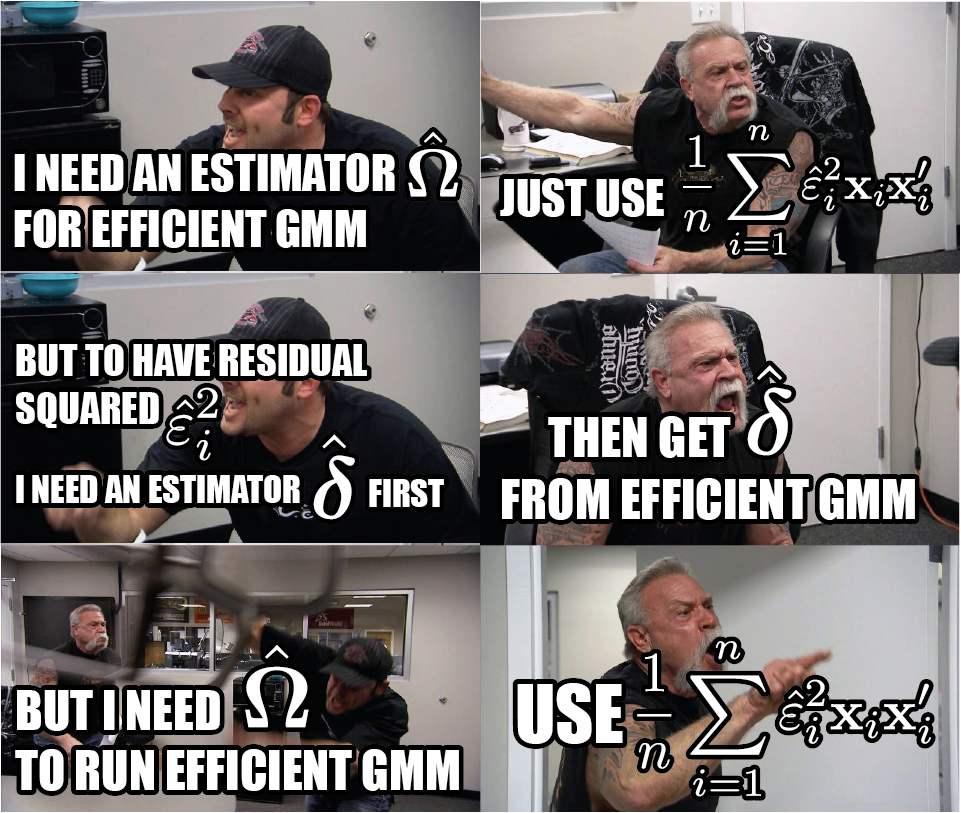
\includegraphics[height=\textheight]{efficient_gmm.png}}
\end{frame}

\begin{frame}{}
	\begin{itemize}
		\item
			However, to obtain a consistent estimator $\hat{\OMEGA}$ for
			$\OMEGA=\E{\varepsilon_i^2\xx_i\xx_i'}$, we need to first obtain a
			consistent estimator for $\ddelta$ since $\hat{\OMEGA}$ is of the
			form
			\begin{align*}
				\hat{\OMEGA} = \frac1n \sum_{i=1}^{n}\hat{\varepsilon}_i^2\xx_i\xx_i'
				\quad\text{where}\quad
				\hat{\varepsilon}_i^2 \coloneqq y_i - \zz_i'\hat{\ddelta}
			\end{align*}
		\item
			Therefore, in practice, there are a number of methods that
			overcomes this problem, either by doing a initial estimation of
			$\ddelta$ first or update $\hat{\WW}$ iteratively.
			\begin{itemize}
				\item \textbf{Two-step feasible GMM}:
					Use $\hat{\WW}=I$ or $\SS_{\xx\xx}\inv$ for the first stage,
					then use the first-stage estimator $\hat{\ddelta}$ to obtain $\hat\OMEGA\inv$.
				\item \textbf{Iterated GMM}:
					Repeat till it converges.
				\item \textbf{Continuously updating GMM}:
					Plug $\WW(\ddelta)=\left(\frac1n\sum_{i=1}^{n}(y_i-\zz_i'\ddelta)\right)\inv$ into $\mathcal{J}$ and minimise it.
			\end{itemize}
	\end{itemize}
\end{frame}

\subsection{How to Check Instruments?}

\begin{frame}{$J$-statistic}
	Checking for instrument validity is very hard.
	Consistent with the GMM idea, the $J$-test is proposed:
	\begin{theorem}[Hansen's test of overidentifying restrictions]
		If all assumptions for GMM hold,
		and there is a consistent estimator for $\OMEGA\inv$,
		then
		\begin{align*}
			\mathcal{J}(\hat{\ddelta}(\hat{\OMEGA}\inv),\hat{\OMEGA}\inv)
			\dto\chi^2_{K-L}
		\end{align*}
	\end{theorem}
	Notice that this test is for \emph{all} assumptions.
	That is, if the test fails, any assumption could be false.
	Furthermore, it is an necessary condition for the validity of the assumptions,
	i.e., even if the test holds, it is not necessary that the assumptions hold.
\end{frame}

\subsection{Implications of Homoskedasticity}

\begin{frame}{Homoskedasticity $\implies$ 2SLS}
	If we impose homoskedasticity, we have
	\begin{align*}
		\E{\varepsilon_i^2\given\xx_i} = \sigma^2
		&\implies \OMEGA = \E{\varepsilon_i^2\xx_i\xx_i'} = \sigma^2\SIGMA_{\xx\xx} \\
		&\implies \hat{\OMEGA} = \frac{\hat{\sigma}^2}{n}\sum_{i=1}^{n}\xx_i\xx_i' = \hat{\sigma}^2\SS_{\xx\xx}
	\end{align*}
	Therefore, the efficient GMM collapses to
	\begin{align*}
		\hat{\ddelta}(\hat{\OMEGA}\inv)
		&= (\SS_{\xx\zz}'(\hat{\sigma}^2\SS_{\xx\xx})\inv\SS_{\xx\zz})\inv\SS_{\xx\zz}'
		(\hat{\sigma}^2\SS_{\xx\xx})\inv\ss_{\xx y} \\
		&= (\SS_{\xx\zz}'\SS_{\xx\xx}\inv\SS_{\xx\zz})\inv\SS_{\xx\zz}'\SS_{\xx\xx}\inv\ss_{\xx y}
		= \hat{\ddelta}(\SS_{\xx\xx}\inv),
	\end{align*}
	which is equivalent to solving the two stage equation
	\begin{align}
		Z = X\beta + \eta &\implies \hat{Z} = X(X'X)\inv X'Z \equiv PZ \\
		Y = \hat{Z}\ddelta + \varepsilon &\implies \hat{\ddelta}_{\text{2SLS}}
			= (Z'P'PZ)\inv{Z'P'Y}
			\equiv \hat{\ddelta}(\SS_{\xx\xx}\inv).
	\end{align}
\end{frame}

\section{Conclusion}

\begin{frame}{Conclusion}
	\begin{itemize}
		\item
			The motivation of GMM comes from generalising the moment conditions
			we use in OLS or IV.
		% \item
		% 	GMM is an umbrella term for many methods.  As we saw earlier, OLS
		% 	and IV can both be regarded as special cases of GMM.
		\item
			Most often in econometric applications, GMM refers to solving
			regressions with more instrument variables than endogenous regressors.
		\item
			GMM is often more computationally intensive, since the minimisation
			process is not very straight forward compared to OLS or IV.
			Nevertheless, it is much more computationally friendly than maximum likelihood.
		\item
			2SLS is implied by homoskedasticity.
	\end{itemize}
\end{frame}

\begin{frame}{References}
	\begin{itemize}
		\item Econometrics (2000) Fumio Hayashi, Chapter 3.
		\item Wikipedia on GMM: \url{https://en.wikipedia.org/wiki/Generalized_method_of_moments}. (largely based on Hayashi)
		\item Wikipedia on Covariance Matrix: \url{https://en.wikipedia.org/wiki/Covariance_matrix}. (definiteness properties of covariance matrix)
	\end{itemize}
\end{frame}

\end{document}
